\section{系統架構設計}

我們參考了 Clean architecture 與 MVVM 來設計架構,引入依賴反轉、雙向數據綁定等特性,旨在減少模組之間的依賴與增加可重用性,使得各部分能獨立開發和測試,並使得未來對系統的修改和擴展更為容易。此外,明確的架構和分層可以幫助團隊成員更快地瞭解專案結構,並減少彼此之間的工作衝突。

\begin{figure}[H]
  \centering
  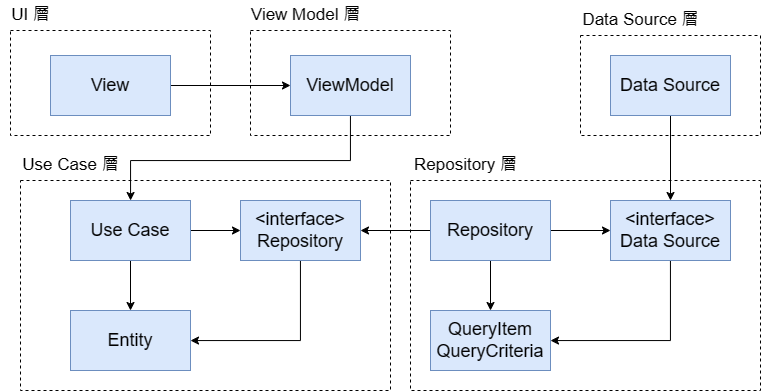
\includegraphics[width=0.8\textwidth]{../assets/TT分層依賴圖.png}
  \caption{系統架構}
  \label{fig:sysarc}
\end{figure}

我們將系統架構分為 Use Case、Repository、Data Source、View Model 和 UI 共五層,分別負責業務邏輯、數據調用、與數據來源溝通、管理 UI 狀態以及呈現使用者介面。圖 1 為分層依賴圖,展示了各層內部的元件與依賴關係。

\begin{itemize}
  \item 資料容器:Entity 為系統中的主要資料結構包含旅程、軌跡、座標點等核心資料,而QueryItem 為向外部資料庫(如 SQL)請求所獲得的原始結果,其欄位與資料表的定義相同
  \item 抽象介面:我們在上層定義下層的介面,並讓下層實作,來達到依賴反轉的目的,如 Repository 與 Data Source 的抽象介面。
  \item 雙向綁定:利用 FluƩer 的 ChangeNoƟfier 實作 MVVM 架構,將 View Model 與 UI 進行雙向數據綁定,並透過 Use Case 處理業務邏輯和數據操作。
\end{itemize}